In questa capitolo si descriverà il problema affrontato per poi passare alle versioni sequenziale e distribuita della soluzione (è possibile trovare le due versioni sulla piattaforma di versioning GitHub), e infine si discuterà delle prestazioni della versione distribuita.
\section{Descrizione del problema}
Il problema affrontato in questo studio riguarda l'applicazione dell'algoritmo \textbf{SIFT}(Scale-Invariant Feature Transform) per effettuare object detection. L' object detection è una tecnologia informatica correlata alla visione artificiale e all'elaborazione di immagini che si occupa di rilevare istanze di oggetti semantici di una determinata classe in immagini e video digitali. Il rilevamento di oggetti ha applicazioni in molte aree della visione artificiale, tra cui il recupero di immagini e la videosorveglianza. Per ogni oggetto in un'immagine, ci sono molte \textbf{features}, che sono caratteristiche interessanti dell'oggetto, le quali possono essere estratte in modo da fornire una descrizione "caratteristica" di quest'ultimo. Questa descrizione estratta da un'immagine campione può poi essere utilizzata per identificare l'oggetto durante il tentativo di individuare l'oggetto in un'immagine contenente più oggetti. Per poter recuperare queste features esistono diversi algoritmi quali per esempio \textbf{SURF}(Speeded Up Robust Features), \textbf{ORB} (Oriented FAST and Rotated BRIEF) e \textbf{SIFT}. In questo studio ci siamo concentrati su quest'ultimo il quale è un algoritmo cpu-intensive e quindi ci interessava analizzare il suo comportamento in un ambiente distribuito.
\subsection{SIFT}
Scale-invariant feature transform (SIFT) è un algoritmo utilizzato in computer vision che permette di rilevare e descrivere caratteristiche pubblicato da David G. Lowe\cite{lowe04} nel 2004. L'algoritmo consiste in un metodo in grado di estrarre delle caratteristiche distintive invarianti da un'immagine che possono essere utilizzate per effettuare un matching tra diversi oggetti. Le caratteristiche sono invarianti rispetto alla scala e alla rotazione dell'immagine e sono mostrate per fornire una robusta corrispondenza su una vasta gamma di distorsioni affini, cambiamenti nel punto di vista 3D, aggiunta di rumore e cambiamento nell'illuminazione. L'algoritmo esegue cinque step:
\begin{enumerate}
	\item \textbf{Scale-space Extrema Detection}
	      Per poter individuare dei keypoints abbiamo bisogno di diverse scale di un immagine quindi viene applicato un filtro per la scala. Questo filtro utilizza la \textbf{Laplaciana di una Gaussiana}(LoG) che permette di rilevare blob di varie dimensioni grazie all'utilizzo di $\sigma$ che funge come parametro di scala. Poichè LoG è costoso SIFT usa la differenza gaussiana(DoG) come alternativa che è una approssimazione del primo. La DoG è ottenuta come differenza di sfocatura gaussiana di un immagine con diversi $\sigma$ (si parte da un valore iniziale di $\sigma$ fino ad arrivare $k\sigma$) . Questo processo viene eseguito per diverse ottave dell'immagine.
	      \begin{figure}[ht]
		      \begin{center}
			      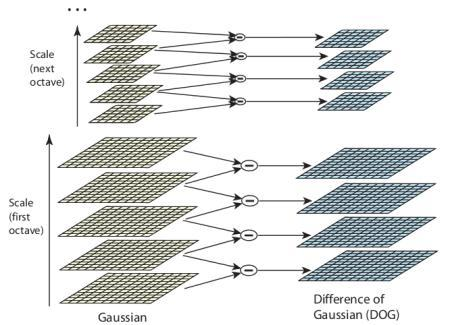
\includegraphics[scale=0.7]{DoG.jpg}
			      \caption{Ottave di un immagine}
			      \label{fig:DoG}
		      \end{center}
	      \end{figure}
	      Una volta trovato DoG vengono cercati i keypoints che rappresentano meglio l'immagine confrontando i pixel su diverse scale, per esempio un pixel in una immagine viene confrontato con i suoi 8 vicini e e con i 9 pixel della scala precedente e successiva.
	      \begin{figure}[ht]
		      \begin{center}
			      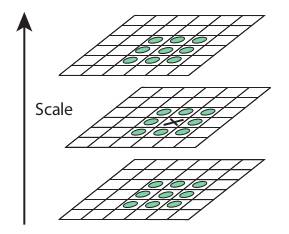
\includegraphics[scale=0.7]{kp.jpg}
			      \caption{Ricerca di un keypoints}
			      \label{fig:kp}
		      \end{center}
	      \end{figure}
	      Il paper fornisce alcuni dati ottimali e sono: numero di ottave = 4, livelli di scala = 5 valore iniziale $\sigma$ = 1.6 e k = $\sqrt{2}$.
	\item \textbf{Keypoint Localization}
	      Una volta individuati potenziali keypoints, devono essere affinati per ottenere risultati più accurati. Viene usata l'espansione della serie di Taylor dello spazio di scala per ottenere una posizione più accurata dei punti e, se l'intensità di un punto è inferiore a un valore di threshold (0,03 valore di soglia del paper), viene rifiutata.
	      La DoG(Difference of Gaussian) ha una risposta più alta per gli edge e che quindi vanno rimossi, per fare questo SIFT usa una matrice Hessiana 2x2 per computare la curvatura per poi confrontarla con la threshold degli edge se viene superata allora gli edge vengono rimossi
	\item \textbf{Orientation Assignment}
	      Successivamente viene assegnato un orientamento a ciascun keypoint per ottenere l'invarianza alla rotazione dell'immagine. Dei vicini vengono presi attorno alla posizione del punto in base alla scala, e al modulo del gradiente e la direzione vengono calcolate in quella regione. Viene creato un istogramma di orientamento con 36 contenitori a 360 gradi. Viene pesato per il modulo del gradiente e la gaussian-weighted circular window con $\sigma$ uguale a 1,5 volte la scala del punto chiave, viene preso il picco più alto nell'istogramma e anche qualsiasi picco superiore a 80 vengono considerati per calcolare l'orientamento.
	\item \textbf{Keypoint Descriptor}
	      In questa fase viene creato un descrittore di keypoint. Viene preso un intorno 16x16 attorno al keypoint. Viene  diviso in 16 sotto blocchi di dimensione 4x4. Per ciascun sottoblocco viene creato un istogramma di orientamento a 8 bin. Quindi sono disponibili in totale 128 valori bin. Questo rappresentato come un vettore per formare un descrittore di keypoints. Oltre a questo, vengono prese diverse misure per ottenere robustezza contro i cambiamenti di illuminazione, la rotazione ecc.
	\item \textbf{Keypoint Matching}
	      I keypoints tra due immagini sono abbinati identificando i loro vicini più vicini. Ma in alcuni casi, la seconda corrispondenza più vicina potrebbe essere molto vicina alla prima. Questo può accadere a causa di rumore o per altri motivi. In questi casi, viene preso il rapporto tra distanza più vicina e distanza più vicina al secondo. Se è maggiore di 0.8, vengono rifiutati. In questo modo si riesco a eliminare circa il 90\% di false corrispondenze mentre scarta solo il 5\% corrispondenze corrette.
\end{enumerate}
\subsection{OpenCV}
Per l'implementazione dell'object detection è stato utilizzato OpenCV. OpenCV (Open Source Computer Vision Library) è una libreria open source di computer vision e di apprendimento automatico, realizzato per fornire un'infrastruttura comune per le applicazioni di visione artificiale e per accelerare l'uso della percezione della macchina nei prodotti commerciali. OpencCV è rilasciato con licenza BSD e la sua libreria ha più di 2500 algoritmi ottimizzati, che comprendono un set completo di algoritmi di visione artificiale e di apprendimento automatico sia classici che all'avanguardia. questi algoritmi possono essere utilizzati per rilevare e riconoscere i volti, identificare gli oggetti, classificare azioni umane nei video, tracciare i movimenti della telecamera, tracciare oggetti in movimento, estrarre modelli 3D di oggetti, trova immagini simili da un database di immagini, rimuovi gli occhi rossi dalle immagini scattate con il flash, segui i movimenti degli occhi, riconosci i paesaggi e stabilisci i marcatori per sovrapporli alla realtà aumentata, ecc. OpenCV supporta diversi linguaggi C++, Python, Java e MATLAB e i pricipali sistemi operativi Linux, Windows Mac os, e Android.
\section{Versione Sequenziale}
Il core della versione sequenziale è il \emph{\textit{SiftManager}}. L'algoritmo prevede l'individuazione di un unico oggetto(query) all'interno di una o più scene(train). Il nostro algoritmo esegue cinque step:
\begin{itemize}
	\item \textbf{Fase Uno :}\\
	Vengono estratte le caratteristiche grazie all'algoritmo SIFT dall'immagine query e dall'immagine di train.
	      Prima vengono estratti i keypoints attraverso \emph{\textit{extractKeypoints}} e successivamente i descrittori con \emph{\textit{extractDescriptors}}
\begin{lstlisting}
public static MatOfKeyPoint extractKeypoints(Mat image, Feature2D extractor) {
  MatOfKeyPoint imageKeypoint = new MatOfKeyPoint();
  extractor.detect(image, imageKeypoint);
  return imageKeypoint;
}
	      
public static MatOfKeyPoint extractDescriptors(Mat image, MatOfKeyPoint imageKeypoints, Feature2D extractor) {
  MatOfKeyPoint imageDescriptors = new MatOfKeyPoint();
  extractor.compute(image, imageKeypoints, imageDescriptors);
  return imageDescriptors;
}
\end{lstlisting}
	\item \textbf{Fase Due :}\\
	Viene effettuato il match tra le immagini query e train utilizzando l'algoritmo di Brute Force e utilizzando knnMatch con k = 2 , dove k indica il conteggio delle migliori corrispondenze trovate per ogni descrittore di query , inoltre viene effettuato anche il \textbf{ratio test} di Lowe (il valore ottimale per il ratio test è 0.75, dal paper di Lowe) sulle distanze dei punti per ogni coppia di match trovato, in modo da filtrare dei possibili falsi positivi.
\begin{lstlisting}
public static MatOfDMatch calculateMatches(MatOfKeyPoint objectDescriptor, MatOfKeyPoint sceneDescriptor, DescriptorMatcher matcher){
  List<MatOfDMatch> knnMatches = new ArrayList<>();
  matcher.knnMatch(objectDescriptor, sceneDescriptor, knnMatches, 2);
  List<DMatch> listOfGoodMatches = new ArrayList<>();
  for (int i = 0; i < knnMatches.size(); i++) {
    if (knnMatches.get(i).rows() > 1) {
      DMatch[] matches = knnMatches.get(i).toArray();
        if (matches[0].distance < RATIO_THRESHOLD * matches[1].distance) {
          listOfGoodMatches.add(matches[0]);
        }
    }
  }
  MatOfDMatch goodMatches = new MatOfDMatch();
  goodMatches.fromList(listOfGoodMatches);
  return goodMatches;
}
\end{lstlisting}
	\item \textbf{Fase Tre :}\\
	Viene rilevato l'oggetto tracciandone calcolandone l'omografia.
\begin{lstlisting}
public static Mat localizeObject(List<KeyPoint> objectKeypoints, List<KeyPoint> sceneKeypoints, MatOfDMatch goodMatches) {
  List<Point> obj = new ArrayList<>();
  List<Point> scene = new ArrayList<>();
  List<DMatch> listOfGoodMatches = goodMatches.toList();
  for (int i = 0; i < listOfGoodMatches.size(); i++) {
    obj.add(objectKeypoints.get(listOfGoodMatches.get(i).queryIdx).pt);
    scene.add(sceneKeypoints.get(listOfGoodMatches.get(i).trainIdx).pt);
  }
  MatOfPoint2f objMat = new MatOfPoint2f(), sceneMat = new MatOfPoint2f();
  objMat.fromList(obj);
  sceneMat.fromList(scene);
  Mat H = Calib3d.findHomography(objMat, sceneMat, Calib3d.RANSAC, RANSAC_THRESHOLD);
  return H;
}
\end{lstlisting}
	\item \textbf{Fase Quattro:}\\
	Si effettua una stima sulla bontà dell'omografia.
\begin{lstlisting}
public static boolean checkHomography(Mat homography){
  double firstCheck = Math.abs(Math.abs(homography.get(0, 0)[0]) - Math.abs(homography.get(1, 1)[0]));
  double secondCheck = Math.abs(Math.abs(homography.get(0, 1)[0]) - Math.abs(homography.get(1, 0)[0]));
  return firstCheck <= 0.1 && secondCheck <= 0.1;
}
\end{lstlisting}
	\item \textbf{Fase Cinque:}\\
	Se la stima avviene con successo si disegna l'immagine in output, mostrando i match e l'omografia.
\begin{lstlisting}
public static Mat drawImage(Mat objectImage, Mat sceneImage, MatOfKeyPoint objectKeypoints, MatOfKeyPoint sceneKeypoints, MatOfDMatch matches, Mat homography) {
  Mat outputImage = new Mat();
  Features2d.drawMatches(objectImage, objectKeypoints, sceneImage, sceneKeypoints, matches, outputImage, Scalar.all(-1),
    Scalar.all(-1), new MatOfByte(), Features2d.NOT_DRAW_SINGLE_POINTS);
  Mat objCorners = new Mat(4, 1, CvType.CV_32FC2), sceneCorners = new Mat();
  float[] objCornersData = new float[(int) (objCorners.total() * objCorners.channels())];
  objCorners.get(0, 0, objCornersData);
  objCornersData[0] = 0;
  objCornersData[1] = 0;
  objCornersData[2] = objectImage.cols();
  objCornersData[3] = 0;
  objCornersData[4] = objectImage.cols();
  objCornersData[5] = objectImage.rows();
  objCornersData[6] = 0;
  objCornersData[7] = objectImage.rows();
  objCorners.put(0, 0, objCornersData);
  Core.perspectiveTransform(objCorners, sceneCorners, homography);
  float[] sceneCornersData = new float[(int) (sceneCorners.total() * sceneCorners.channels())];
  sceneCorners.get(0, 0, sceneCornersData);
  Imgproc.line(outputImage, new Point(sceneCornersData[0] + objectImage.cols(), sceneCornersData[1]),
    new Point(sceneCornersData[2] + objectImage.cols(), sceneCornersData[3]), RECT_SCALAR, 4);
  Imgproc.line(outputImage, new Point(sceneCornersData[2] + objectImage.cols(), sceneCornersData[3]),
    new Point(sceneCornersData[4] + objectImage.cols(), sceneCornersData[5]), RECT_SCALAR, 4);
  Imgproc.line(outputImage, new Point(sceneCornersData[4] + objectImage.cols(), sceneCornersData[5]),
    new Point(sceneCornersData[6] + objectImage.cols(), sceneCornersData[7]), RECT_SCALAR, 4);
  Imgproc.line(outputImage, new Point(sceneCornersData[6] + objectImage.cols(), sceneCornersData[7]),
    new Point(sceneCornersData[0] + objectImage.cols(), sceneCornersData[1]), RECT_SCALAR, 4);
  return outputImage;
}
\end{lstlisting}
	      \begin{figure}[H]
		      \begin{center}
			      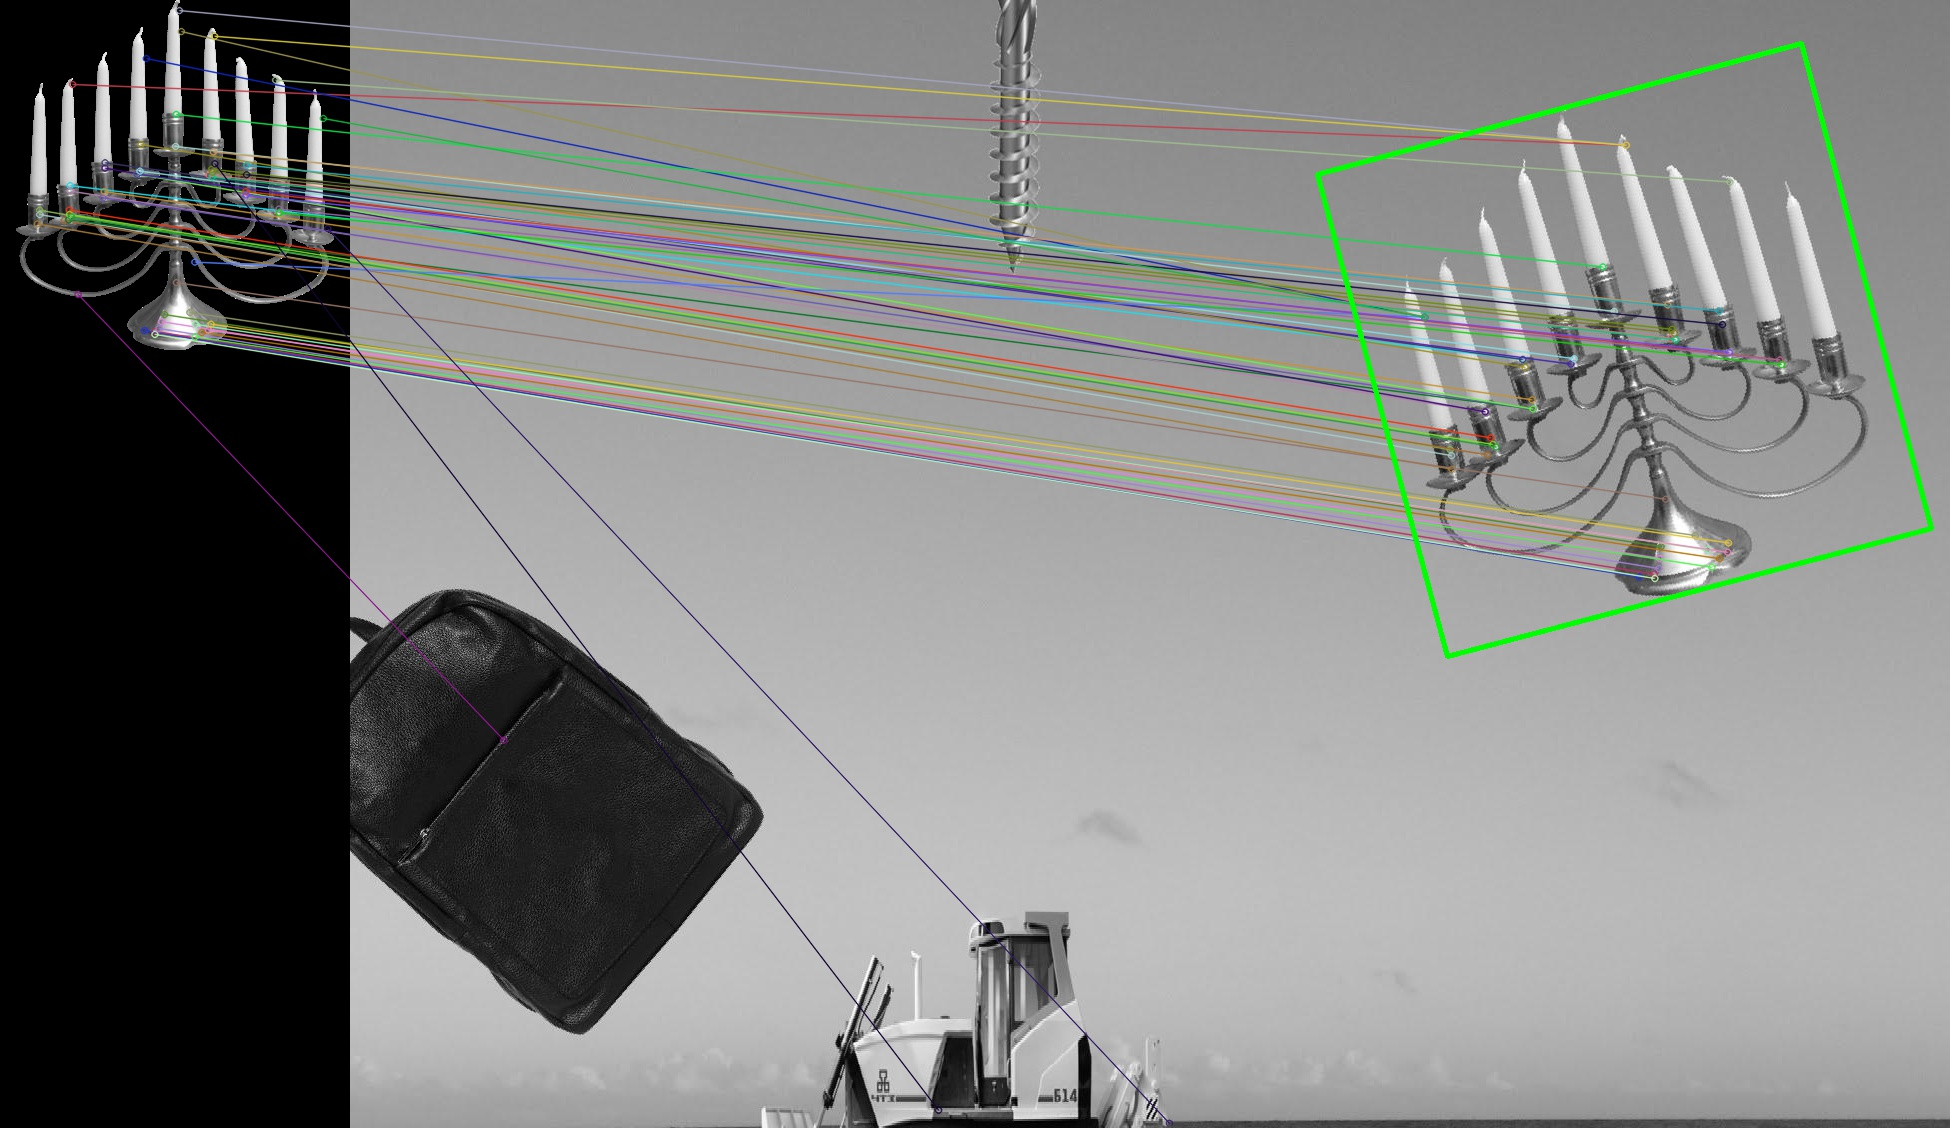
\includegraphics[width=\linewidth]{omografia.jpg}
			      \caption{Esempio di esito positivo}
			      \label{fg:omografia.jpg}
		      \end{center}
	      \end{figure}
\end{itemize}
\section{Versione Distibuita con Hadoop}
La versione distribuita funziona nel seguente modo, prese una serie di immagini query(oggetto da cercare) e una serie di train(scene) ogni oggetto viene cercato in tutte le scene. Il core resta lo stesso visto precedentemente in \emph{\textit{SiftManager}} ma vengono aggiunti \emph{\textit{SiftUtilis}} che presenta delle funzioni di supporto per le diverse conversione necessarie per poter effettuare il trasferimento di immagini su Hadoop, \emph{\textit{SiftReduce}} per il reduce sul cluster di Hadoop, \emph{\textit{SiftMapper}} per il mapping ,\emph{\textit{MatWritable}} e \emph{\textit{MatOfKeyPointWritable}} per serializzare il risultato ottenuto dal map e poterlo passare al reduce.
\begin{itemize}
	\item \textbf{Map}:\\
	      Il Map si occupa di estrarre i descrittori nei diversi oggetti da cercare successivamente nelle scene
\begin{lstlisting}
@Override
protected void map(Text key, MatWritable value, Context context) throws IOException, InterruptedException {
  SIFT sift = SIFT.create();
  SiftManager manager = SiftManager.getInstance();
  MatOfKeyPoint objectKeyPoints = manager.extractKeypoints(value.getImage(), sift);
  MatOfKeyPoint objectDescriptors = manager.extractDescriptors(value.getImage(), objectKeyPoints, sift);
  MapWritable map = new MapWritable();
  map.put(new Text(SiftUtils.OBJ_IMG), value);
  map.put(new Text(SiftUtils.OBJ_KPS), new MatOfKeyPointWritable(objectKeyPoints));
  map.put(new Text(SiftUtils.OBJ_DSC), new MatOfKeyPointWritable(objectDescriptors));
  context.write(key, map);
}
\end{lstlisting}

	\item \textbf{Reduce}:\\
	      Il Reduce ha il compito di estrarre i descrittori della scena e successivamente di effettuare il match tra l'oggetto e la scena
\begin{lstlisting}
protected void reduce(Text key, Iterable<MapWritable> values, Context context) throws IOException, InterruptedException {
  for (MapWritable map : values) {
    MatWritable receivedImage = ((MatWritable) map.get(new Text(SiftUtils.OBJ_IMG)));
    MatOfKeyPointWritable receivedKeyPoints = ((MatOfKeyPointWritable) map.get(new Text(SiftUtils.OBJ_KPS)));
    MatOfKeyPointWritable receivedObjectDescriptors = ((MatOfKeyPointWritable) map.get(new Text(SiftUtils.OBJ_DSC)));
    MatOfKeyPoint objectDescriptors = receivedObjectDescriptors.getMatOfKeyPoint();
    MatOfKeyPoint objectKeypoints = receivedKeyPoints.getMatOfKeyPoint();
    FileSystem fs = FileSystem.get(context.getConfiguration());
    Path scenePath = Path.mergePaths(fs.getHomeDirectory(), new Path("/scenes"));
    RemoteIterator iterator = fs.listLocatedStatus(scenePath);
    while (iterator.hasNext()) {
      LocatedFileStatus lfs = (LocatedFileStatus) iterator.next();
      String format = SiftUtils.extractFormat(lfs.getPath().getName());
      String name = lfs.getPath().getName().substring(0, lfs.getPath().getName().lastIndexOf("."));
      if (lfs.isFile()) {
        InputStream input = fs.open(lfs.getPath());
        Mat sceneImg = SiftUtils.readInputStreamIntoMat(input);
        MatOfKeyPoint sceneKeyPoints = SiftManager.extractKeypoints(sceneImg, sift);
        MatOfKeyPoint sceneDescriptors = SiftManager.extractDescriptors(sceneImg, sceneKeyPoints, sift);
        MatOfDMatch matches = SiftManager.calculateMatches(objectDescriptors, sceneDescriptors, descriptor);
        if (!matches.empty()) {
          Mat homography = SiftManager.localizeObject(objectKeypoints.toList(), sceneKeyPoints.toList(), matches);
            if (SiftManager.checkHomography(homography)) {
              Mat outputImg = SiftManager.drawImage(receivedImage.getImage(), sceneImg, objectKeypoints,
                sceneKeyPoints, matches, homography);
                context.write(key, new MatWritable(outputImg, name, format));
            }
          }
        }
      }
      fs.close();
    }
  }
}
\end{lstlisting}

	\item  \textbf{SiftUtilis}:\\
Poichè Hadoop lavora su stream di byte e OpenCV per rappresentare le immagini usa oggetti di tipo Mat, si è reso necessario la creazioni di due metodi,  e \emph{\textit{byteToMat}}, per poter effettuare la conversione da Mat a byte e viceversa
\begin{lstlisting}
public static int totalSize(Mat image){
  return Math.toIntExact(image.total()) * image.channels();
}

public static byte[] matToByte(Mat image){
  byte[] bytes = new byte[SiftUtils.totalSize(image)];
  image.get(0, 0, bytes);
  return bytes;
}

public static Mat byteToMat(byte[] bytes, int width, int height, int type){
  Mat image = new Mat(height, width, type);
  image.put(0, 0, bytes);
  return image;
}
\end{lstlisting}
Per poter leggere le immagini passate dal reduce bisogna convertirle in Mat \emph{\textit{readInputStreamIntoMat}}
\begin{lstlisting}
private static byte[] readStream(InputStream stream) throws IOException {
  ByteArrayOutputStream buffer = new ByteArrayOutputStream();
  int nRead;
  byte[] data = new byte[16384];
  while ((nRead = stream.read(data, 0, data.length)) != -1) {
    buffer.write(data, 0, nRead);
  }
  buffer.flush();
  byte[] temporaryImageInMemory = buffer.toByteArray();
  buffer.close();
  stream.close();
  return temporaryImageInMemory;
}

public static Mat readInputStreamIntoMat(InputStream inputStream) throws IOException {
  byte[] temporaryImageInMemory = readStream(inputStream);
  Mat outputImage = Imgcodecs.imdecode(new MatOfByte(temporaryImageInMemory), Imgcodecs.CV_LOAD_IMAGE_GRAYSCALE);
  return outputImage;
}
\end{lstlisting}
\end{itemize}
\section{Analisi delle prestazioni}
Analizzare le prestazioni di un applicativo parallelo significa eseguire dei \textbf{Test di Performance} e quindi bisogna eseguire un approccio preciso e deterministico sulla sua esecuzione. Questo test si occuperà di raggiungere due obiettivi: scalabilità della soluzione, correttezza dell'algoritmo. Per quanto riguarda il primo obiettivo definiamo come scalabilità la capacità di un sistema di adattarsi al carico di lavoro che riceve e in questo test, si è ritenuto opportuno focalizzarsi sulla \textbf{Strong Scalability} ossia verificare che all'aumentare della potenza di calcolo, mantenendo lo stesso carico di lavoro, i tempi di risposta dell'algoritmo diminuiscano. Aumentare la potenza di calcolo in un cluster Hadoop comporta due operazioni da fare: aumentare il numero di slave e di reduce task da eseguire rispettivamente effettuando operazioni di commissioning/decomissioning dei nodi e modificando i parametri dell'applicativo. Il secondo obiettivo si ramifica in due sotto obiettivi: verificare che SIFT individui gli oggetti nella scena indipendentemente da qualunque trasformazione essi possano subire, e scartare il maggior numero possibile di falsi positivi. La generazione del dataset è stata pianificata per andare incontro a queste esigenze ed è stata effettuata nel seguente modo:
\begin{enumerate}
	\item Sono stati prelevati dalla rete 150 oggetti (quasi sempre due della stessa tipologia) ad alta risoluzione;
	\item Grazie ad uno script Python scritto ad hoc sono state generate 5000 immagini ad alta definizione dove 4 oggetti vengono posizionati all'interno di uno sfondo (un cielo) in maniera casuale dove a due di essi è stata sottoposta una rotazione che può variare dai 0 a 180 gradi mentre ai rimanenti una ridimensionamento che può variare dal 15\% al 50\%;
	\item Il posizionamento casuale non avviene rispettando che l'oggetto debba essere completamente visibile in scena. Infatti può avvenire che alcuni oggetti si sovrappongano o che una parte esca fuori dalla scena in modo da creare un effetto di "occultamento" e testare anche la capacità di individuazione in ambiente occluso;
\end{enumerate}
\subsection{Sistema}
I test sono stati effettuati su un cluster fornito dal GARR composto da 24 nodi ognuno con le seguenti caratteristiche:
\begin{table}[H]
	\begin{tabular}{|c|c|}
		\hline
		\multicolumn{2}{|c|}{\textbf{Hardware}} \\
		\hline
		Intel Xeon E3-12xx v2 & x8              \\
		\hline
		Ram                   & 32GB            \\
		\hline
		Scrittura Disco       & 3.1 GB/s        \\
		\hline
		Lettura               & 3.5GB/s         \\
		\hline
	\end{tabular}
	\hfill
	\begin{tabular}{|c|c|}
		\hline
		\multicolumn{2}{|c|}{\textbf{Software}} \\
		\hline
		Sistema Operativo & 16.04.04            \\
		\hline
		Linux             & 4.4.0               \\
		\hline
		Java              & 8.0                 \\
		\hline
		Hadoop            & 2.7.3               \\
		\hline
	\end{tabular}
	\caption{Tabelle Configurazioni}
\end{table}
CPU e RAM sono state recuperane con il comando \textit{lshw} mentre kernel e sistema operativo col comando \textit{uname}. Le versioni di Java e di Hadoop sono state recuperate con gli appositi comandi forniti da entrambi i software mentre per i parametri di lettura e scrittura del disco sono stati eseguiti i seguenti comandi unix:
\begin{lstlisting}
// scrittura
sync; dd if=/dev/zero of=tempfile bs=1M count=1024; sync
// lettura
dd if=tempfile of=/dev/null bs=1M count=1024
\end{lstlisting}
\subsection{Configurazioni}
La configurazione del cluster è la parte più importante affinchè hadoop utilizzi al meglio le risorse disponibili ed è necessario configurare 3 file:
\begin{itemize}
	\item hdfs-site.xml;
	\item yarn-site.xml;
	\item mapred-site.xml
\end{itemize}
Per quanto riguarda il primo file, esso contiene le informazioni necessarie per configurare i parametri dell'HDFS. Si è preferito lasciare la size dei blocchi a 64MB e nessun fattore di replicazione in quanto non vogliamo che si perda del tempo di CPU e di scritture sul disco. Il secondo file è invece il gestore delle risorse dove vengono allocati RAM e CPU per i container. Si è deciso di assegnare 30 sui 32GB di RAM ai container questo perché è necessario lasciare della memoria al sistema operativo ed essendo non provvisto di interfaccia grafica riteniamo che 2GB siano più che sufficienti. Per quanto riguarda le risorse da destinare ai container si è optato per un totale di 4 container per slave dove ognuno di essi ha da un minimo di 4 ad un massimo di 7GB di RAM disponibile ed un minimo di 2 ad un massimo di 7 core disponibili. L'ultimo file è quello per la configurazione delle risorse dei map-reduce e alla luce dei parametri assegnati a YARN si è deciso di assegnare un limite superiore di 4GB per i map e 7GB per i reduce. Essendo che ogni container alloca un processo Java è necessario impostare anche la size necessaria all'heap di java per ogni task e si è giunti alla conclusione che una politica aggressiva di un 80\% della RAM dei map e dei reduce, sia adeguata per fare fronte al problema. Per riassumere ecco le configurazioni utilizzate:
\begin{table}[H]
	\begin{center}
		\begin{tabular}{ | c | c |}
			\hline
			\textbf{Opzione YARN}                    & \textbf{Valore} \\
			\hline
			yarn.nodemanager.resource.memory-mb      & 30720           \\
			\hline
			yarn.nodemanager.resource.cpu-vcores     & 8               \\
			\hline
			yarn.scheduler.minimum-allocation-vcores & 2               \\
			\hline
			yarn.scheduler.maximum-allocation-vcores & 4               \\
			\hline
			yarn.scheduler.minimum-allocation-mb     & 4096            \\
			\hline
			yarn.scheduler.maximum-allocation-mb     & 7168            \\
			\hline
		\end{tabular}
		\caption{Configurazione di \textit{yarn-site.xml}}
	\end{center}
\end{table}
\begin{table}[H]
	\begin{center}
		\begin{tabular}{ | c | c |}
			\hline
			\textbf{Opzione MapReduce}  & \textbf{Valore} \\
			\hline
			mapreduce.map.memory.mb     & 4096            \\
			\hline
			mapreduce.reduce.memory.mb  & 7168            \\
			\hline
			mapreduce.map.java.opts     & -Xmx3276M       \\
			\hline
			mapreduce.reduce.java.opts  & -Xmx5734M       \\
			\hline
			mapreduce.map.cpu.vcores    & 2               \\
			\hline
			mapreduce.reduce.cpu.vcores & 2               \\
			\hline
		\end{tabular}
		\caption{Configurazione di \textit{mapred-site.xml}}
	\end{center}
\end{table}
\begin{table}[H]
	\begin{center}
		\begin{tabular}{ | c | c |}
			\hline
			\textbf{Opzione HDFS} & \textbf{Valore} \\
			\hline
			dfs.replication       & 1               \\
			\hline
			dfs.blocksize         & 64m             \\
			\hline
		\end{tabular}
		\caption{Configurazione di \textit{hdfs-site.xml}}
	\end{center}
\end{table}
\subsection{Impiego delle risorse}
Una volta lancianti i test, sono stati prelevati i dati delle risorse impiegate dai vari slave, tramite il comando \textit{dstat}. Questo comando monitora in background le risorse di una macchina linux e a seconda delle opzioni impostate, si decide cosa monitorare. Per il nostro test sono state monitorate le seguenti informazioni:
\begin{itemize}
\item CPU (percentuale di utilizzo da parte dell'utente, del sistema e in idle);
\item DISCO (letture e scritture);
\item RAM (usata, in cache, libera, nel buffer);
\item SWAP (usata, libera);
\item RETE (pacchetti spediti, inviati);
\end{itemize}
I dati vengono scritti all' interno di un file in formato csv. Una volta che i test sono finiti sono stati prelevati da ogni slave, inseriti all'interno di un database locale (nel nostro caso abbiamo usato MS Access per velocizzare il processo di acquisizione e analisi delle informazioni) ed è stata applicata una semplice media aritmetica sulle colonne per analizzare l'andamento delle risorse e infine, ogni valore è stato infine posizionato su di un grafico a barre.
\subsubsection{CPU}
La prima tripletta di grafici rappresenta l'uso della CPU per i vari test. Sull'asse delle ascisse sono rappresentati ogni slave coinvolto nel test e sull'asse delle ordinate è rappresentata la percentuale di utilizzo della CPU (da un minimo di 0 ad un massimo del 100\%) classificata per uso da parte dell'utente, del sistema, in idle o in attesa. I grafici riportano le seguenti informazioni: Per ogni test lanciato con diverso numero di slave, risulta che solo 4 di essi utilizzino al pieno la quantità di CPU assegnata. Riteniamo che questo sia dovuto alle dimensioni del dataset non adeguate (appena un 1GB) e quindi con la presenza di sovraccarico di comunicazione. Gli stessi valori si presentano sia nel test a 16 slave che in quello a 24 ma questo non implica che la soluzione non scali infatti nei grafici successivi sulle prestazioni del disco si evince chiaramente come tutti gli slave scrivano in parallelo.
\begin{figure}[H]
	\begin{center}
		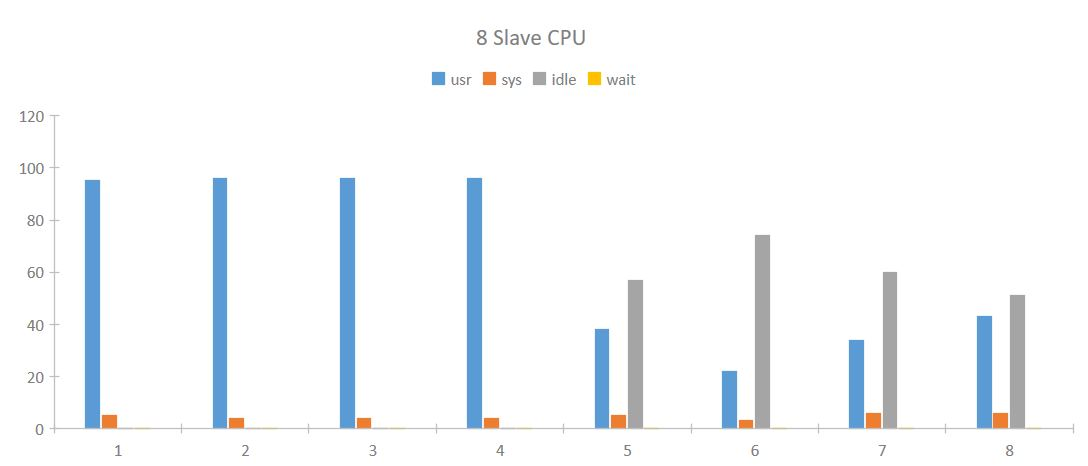
\includegraphics[scale=0.5]{8slavecpu.jpg}
		\caption{Consumo CPU 8 Slave}
		\label{fg:8slavecpu.jpg}
	\end{center}
\end{figure}

\begin{figure}[H]
	\begin{center}
		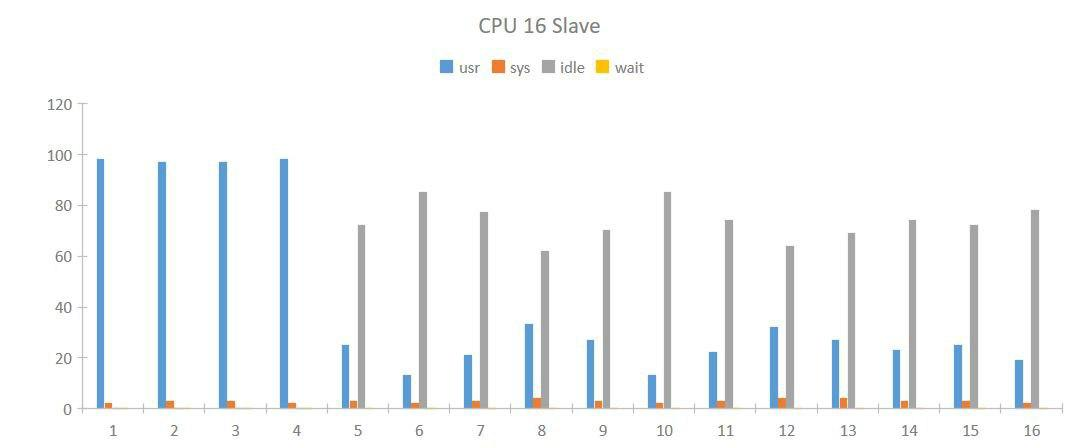
\includegraphics[scale=0.5]{16slavecpu.jpg}
		\caption{Consumo CPU 16 Slave}
		\label{fg:16slavecpu.jpg}
	\end{center}
\end{figure}

\begin{figure}[H]
	\begin{center}
		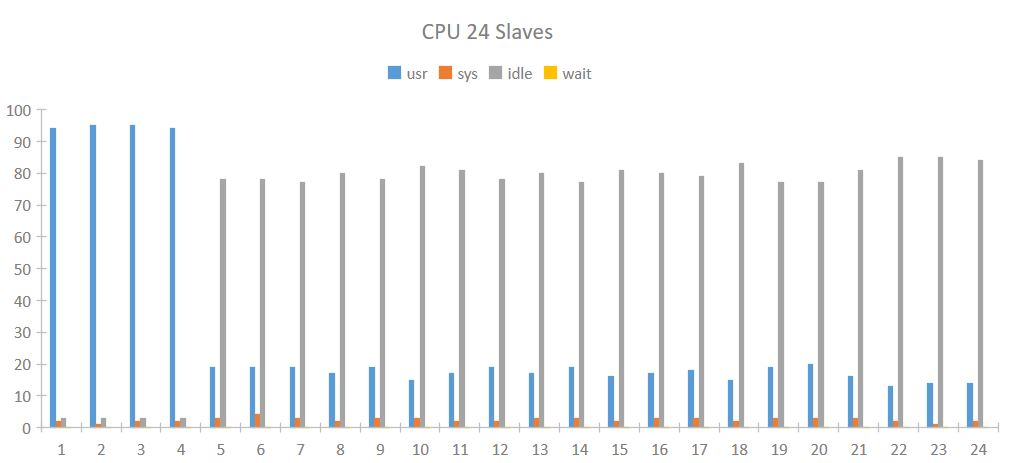
\includegraphics[scale=0.5]{24slavecpu.jpg}
		\caption{Consumo CPU 24 Slave}
		\label{fg:24slavecpu.jpg}
	\end{center}
\end{figure}

\subsubsection{Disco}
La seconda tripletta di grafici illustra l'uso del disco attraverso i vari test. Sull'asse delle ascisse sono riportati gli slave coinvolti nel test mentre sull'asse delle ordinate il numero di byte scritti e letti da ogni slave. Per quanto riguarda l'uso del disco i valori sono quelli previsti: Per ogni test tutti gli slave hanno valori di scrittura alti e bassi in lettura favorendo quindi la località dei dati e scrivendo le immagini che risultano positive sul disco. chi fa parzialmente eccezione è l'ultimo test con 24 slave dove è presente su alcuni nodi una percentuale di lettura più alta. Riteniamo che questo sia dovuto al fatto che i dati in questa configurazione sono più sparsi ed è necessario che gli slave li richiedano per eseguire i reduce task.
\begin{figure}[H]
	\begin{center}
		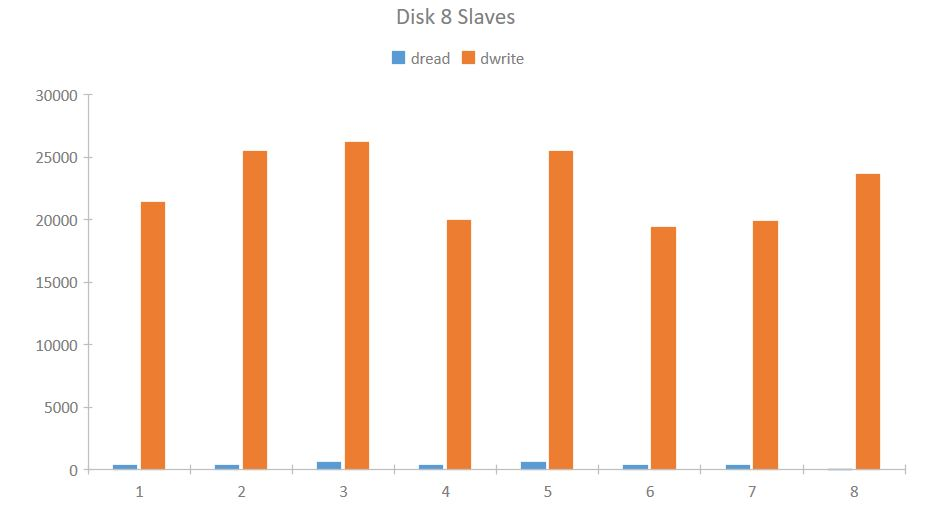
\includegraphics[scale=0.5]{8slavedisk.JPG}
		\caption{Uso del disco 8 Slave}
		\label{fg:8slavedisk.jpg}
	\end{center}
\end{figure}

\begin{figure}[H]
	\begin{center}
		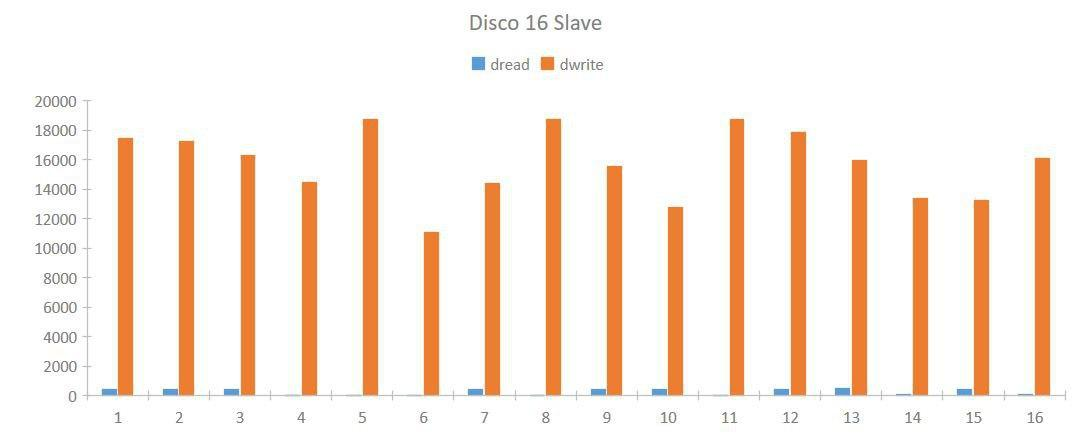
\includegraphics[scale=0.5]{16slavedisk.jpg}
		\caption{Uso del disco 16 Slave}
		\label{fg:16slavedisk.jpg}
	\end{center}
\end{figure}

\begin{figure}[H]
	\begin{center}
		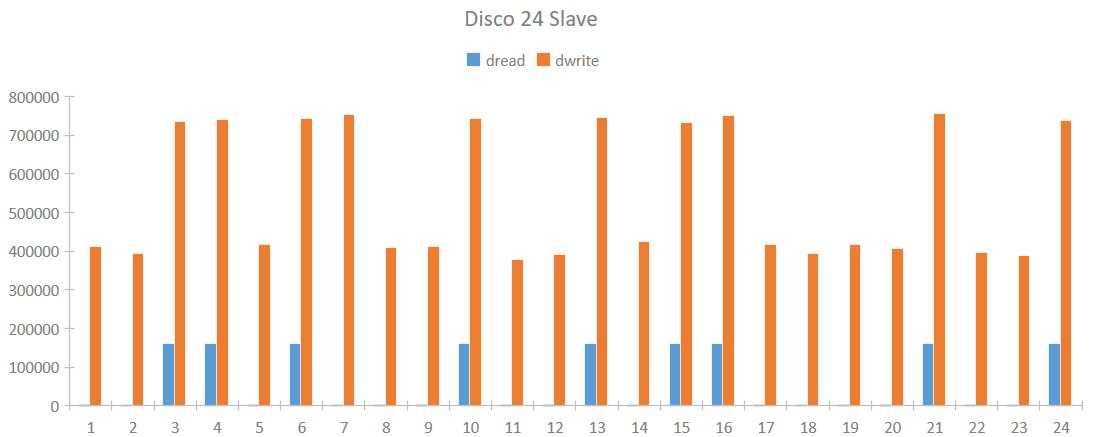
\includegraphics[scale=0.5]{24slavedisk.JPG}
		\caption{Uso del disco 24 Slave}
		\label{fg:24slavedisk.jpg}
	\end{center}
\end{figure}

\subsubsection{Memoria}
In questa tripletta si analizza il consumo di memoria RAM nei test. Sull'asse delle ascisse sono mostrati tutti gli slave coinvolti nel test mentre sull'asse delle ordinate è disposto il consumo di RAM espesso in bytes (si devono dividere per $1024^2$) il tutto classificato per memoria utilizzata, libera, in cache e nel buffer. Dal grafico risulta che l'uso della memoria da parte degli slave non è alta e questo è sicuramente dovuto alle dimensioni del dataset esigue.
\begin{figure}[H]
	\begin{center}
		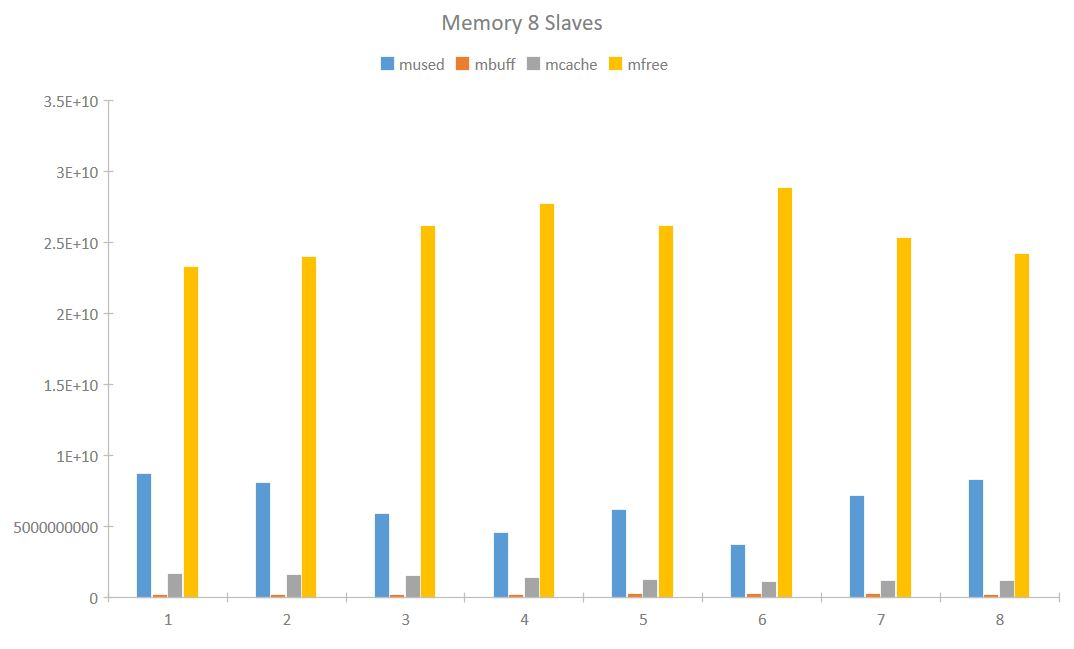
\includegraphics[scale=0.5]{8slavememory.JPG}
		\caption{Utilizzo RAM 8 Slave}
		\label{fg:8slavememory.JPG}
	\end{center}
\end{figure}

\begin{figure}[H]
	\begin{center}
		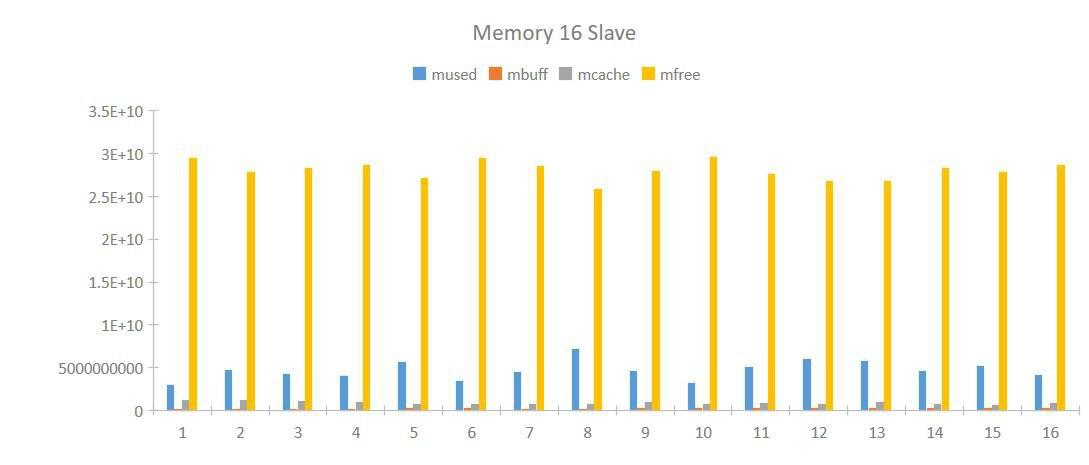
\includegraphics[scale=0.5]{16slavememory.jpg}
		\caption{Utilizzo RAM 16 Slave}
		\label{fg:16slavememory.JPG}
	\end{center}
\end{figure}

\begin{figure}[H]
	\begin{center}
		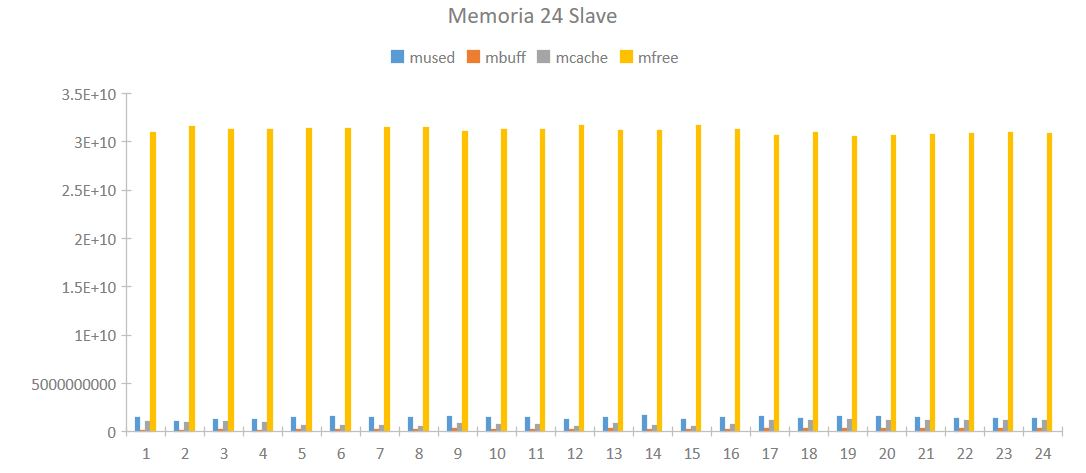
\includegraphics[scale=0.5]{24slavememory.JPG}
		\caption{Utilizzo RAM 24 Slave}
		\label{fg:24slavememory.JPG}
	\end{center}
\end{figure}

\subsubsection{Rete}
L'ultima tripletta rappresenta l'uso della rete nei test. Sull'asse delle ascisse sono riportati gli slave coinvolti nel test mentre sull'asse delle ordinate il numero di byte inviati e ricevuti dai vari slave e classificati per byte e per pacchetti sia inviati che ricevuti. L'uso della rete in tutti i test è molto elevato e questo è dovuto soprattutto perché nella fase di reduce bisogna recuperare dall'HDFS tutte le immagini per poter effettuare i match necessari per l'individuazione ed anche perché tra i map e i reduce viene passata una tripletta di dati serializzati ovvero i keypoint, i descrittori e l'intera immagine da cercare per poter infine scrivere su disco l'immagine con il match individuato.

\begin{figure}[H]
	\begin{center}
		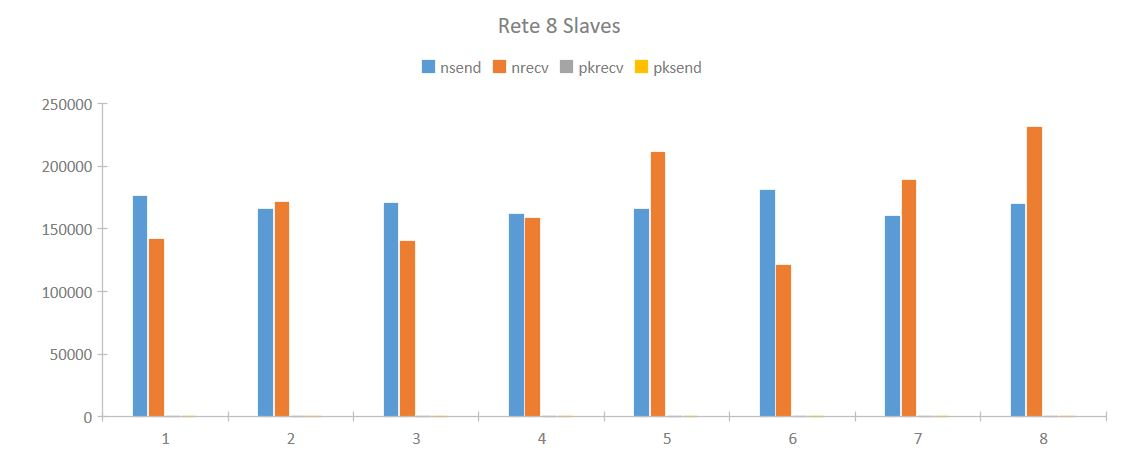
\includegraphics[scale=0.5]{8slavenet.JPG}
		\caption{Utilizzo Rete 8 Slave}
		\label{fg:8slavenet.JPG}
	\end{center}
\end{figure}

\begin{figure}[H]
	\begin{center}
		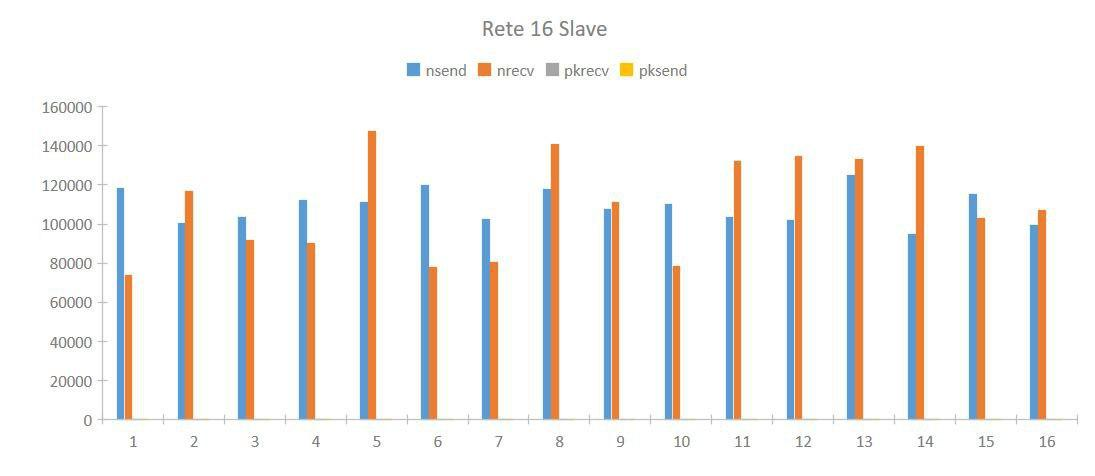
\includegraphics[scale=0.5]{16slavenet.jpg}
		\caption{Utilizzo Rete 16 Slave}
		\label{fg:16slavenet.JPG}
	\end{center}
\end{figure}

\begin{figure}[H]
	\begin{center}
		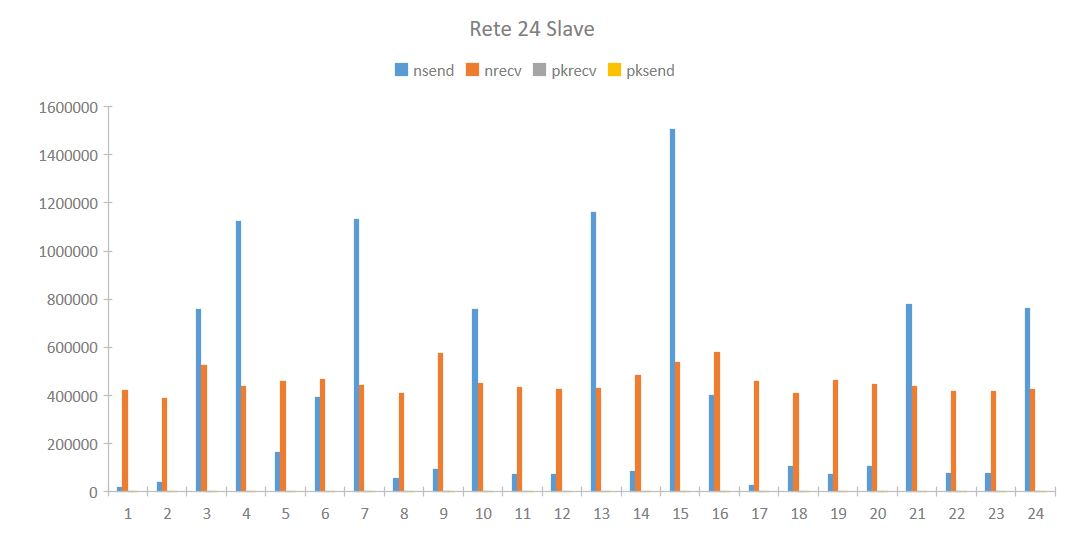
\includegraphics[scale=0.5]{24slavenet.JPG}
		\caption{Utilizzo Rete 24 Slave}
		\label{fg:24slavenet.JPG}
	\end{center}
\end{figure}

\subsection{Risultati delle API REST}
Vengono di seguito riportati i risultati delle API fornite dalla dashboard di Hadoop. Questi ultimi vengono forniti sfruttando i \textbf{Counter} che sono dei veri e propri contatori utili per raccogliere dati e per effettuare del debug basico. Le sezioni che mostra sono informazioni inerenti il file system (locale e distribuito), inerenti ai job, al map reduce e alla fase di shuffle. In tutti i test si notano dei job killed e alcuni failed che sono però "fasulli": nel primo caso alcuni job vengono uccisi a causa della \textbf{Speculative Execution} ovvero Hadoop esegue alcuni task su più slave e quando il primo finisce, causa l'uccisione degli altri in quanto non più necessari. Nel secondo caso i job non falliscono ma il counter viene incrementato in quanto la memoria assegnata al task occupava tutta quella fisica dello slave senza eccedere e il framework è configurato per segnalare questo problema.

\begin{figure}[H]
	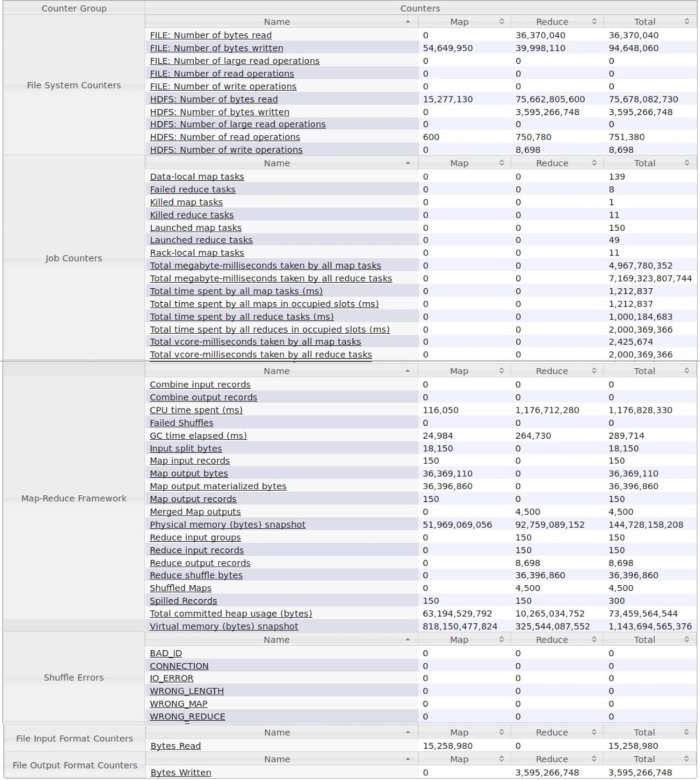
\includegraphics[scale=0.7]{8Slaves.jpg}
	\caption{Counter 8 Slave}
	\label{fg:8Slaves.jpg}
\end{figure}

\begin{figure}[H]
	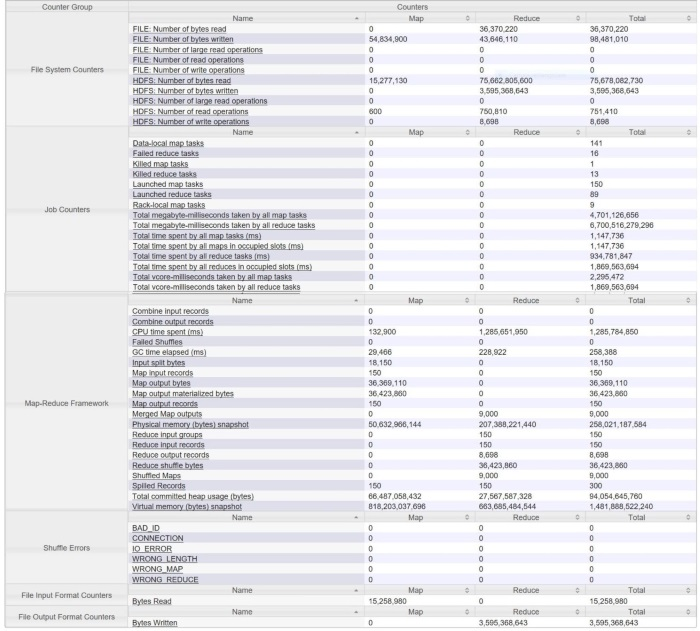
\includegraphics[scale=0.7]{16Slaves.jpg}
	\caption{Counter 16 Slave}
	\label{fg:16Slaves.jpg}
\end{figure}

\begin{figure}[H]
	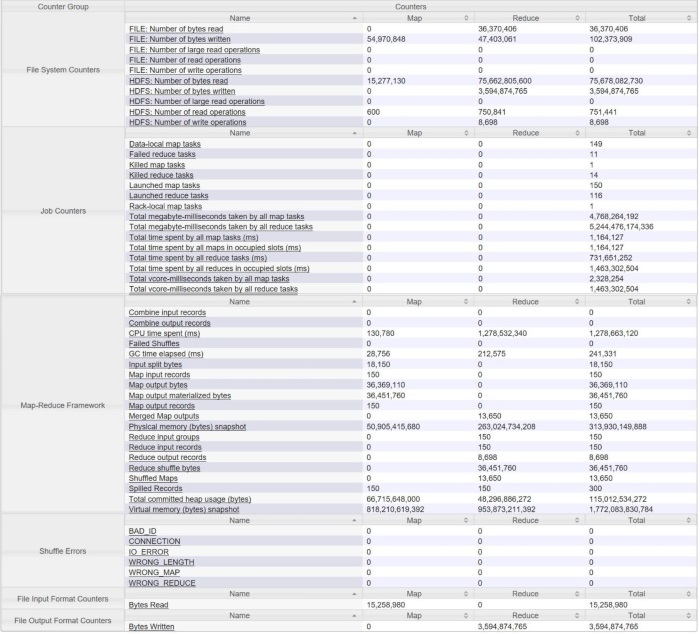
\includegraphics[scale=0.7]{24Slaves.jpg}
	\label{fg:24Slaves.jpg}
	\caption{Counter 24 Slave}
\end{figure}

\subsection{Output dei Test}
Sui 750000 match effettuati dall'algoritmo sono state scritte sul disco un totale di 4570 immagini con meno di 20\% falsi positivi. L'algoritmo riesce ad individuare le immagini in tutte le possibili trasformazioni supposte e inoltre anche quando l'immagine è parzialmente o totalmente occulta. Questo risultato è interessante in quanto siamo riusciti ad ottenere un livello di precisione elevato senza ricorrere a tecniche più complesse basate su autoapprendimento. 

\subsection{Riepilogo finale}
Di seguito sono riportati i tempi presi dalla dashboard di Hadoop e dalla funzione \textit{time}:
\begin{table}
	\begin{center}
		\begin{tabular}{|c|c|c|}
			\hline
			Slave/Tempo & Time(Elapsed) & Hadoop       \\
			\hline
			8 Slave     & 13h, 1m, 20s  & 13h, 54s     \\
			\hline
			16 Slave    & 7h, 19m, 42s  & 7h, 19m, 17s \\
			\hline
			24 Salve    & 5h, 26m, 18s  & 5h, 26m, 3s  \\
			\hline
		\end{tabular}
		\caption{Tabella Tempi di Esecuzione}
	\end{center}
\end{table}
La tabella mostra chiaramente che i tempi differiscono nell'ordine dei secondi ed è normale perchè la time impiega un delta di tempo maggiore per stampare il tutto su standard output.